\documentclass[a4paper, 11pt]{article}
\title{BugBoard 2026}
\author{Marco Festa, Alessandro Giglio, Pierluigi Frascogna}

\usepackage[a4paper, margin=2.5cm, headheight=39pt]{geometry}
\usepackage[italian]{babel}
\usepackage{graphicx}
\usepackage{svg}
\usepackage[table]{xcolor}
\usepackage{tabularx}
\usepackage{multirow}
\usepackage{float}
\usepackage{fancyhdr}
\usepackage{array}
\usepackage{hyperref}

\renewcommand{\arraystretch}{1.4}
\graphicspath{{images/}}
\svgpath{{images/}}
\pagestyle{fancy}
\fancyhf{}  % cancella header/footer di default di Latex
\fancyhead[L]{{\includesvg[height=1.2cm]{BugBoard26_Logo}}} 
\fancyhead[R]{Pag. \thepage} 


\begin{document}

\begin{titlepage}
    \centering
    {\LARGE UNIVERSITÀ DEGLI STUDI FEDERICO II} \\[1em]
    {\large SCUOLA POLITECNICA E DELLE SCIENZE DI BASE} \\[0.5em]
    {\small DIPARTIMENTO DI INGEGNERIA ELETTRICA E TECNOLOGIE DELL'INFORMAZIONE} \\[2em]

    \includesvg[width=0.50\linewidth]{Federico_II_Logo} \\[2em]

    {\large CORSO DI LAUREA IN INFORMATICA} \\[0.5em]
    {\large INSEGNAMENTO DI INGEGNERIA DEL SOFTWARE} \\[2em]

    {\large ANNO ACCADEMICO 2025/2026} \\[2em]

    {\LARGE \textbf{Progettazione e sviluppo della piattaforma BugBoard26}}
\end{titlepage}

\newpage
\tableofcontents  % INDICE

% Qua andrebbo il glossario

\newpage
\section{INTRODUZIONE}

\subsection{Chi siamo}

Benvenuto su \textbf{BugBoard26}! \\
BugBoard26 è una piattaforma di \textit{issues handling} che fornisce una soluzione unica per:
\begin{itemize}
    \item Dividere in modo facile developer in progetti.
    \item Segnalare e gestire intuitivamente issue di vario tipo.
    \item Gestire in modo efficiente tutte le persone coinvolte in un progetto (anche non sviluppatori) tramite una gerarchia di utenze.
\end{itemize}


\newpage
\section{INGEGNERIA DEI REQUISITI}

\subsection{Casi d'uso}
In questa sezione ci interesseremo all'individuazione dei casi d'uso. Come si può evincere dallo use case diagram riportato qui di seguito:

\begin{figure}[H]
    \centering
    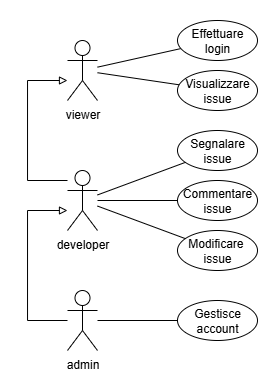
\includegraphics[width=0.5\linewidth]{UseCase_Diagram}
    \caption{Use Case Diagram}
    \label{fig:use_case_diagram}
\end{figure}

Tutti gli utilizzatori della piattaforma possono essere divisi in tre grandi macrocategorie:
\begin{itemize}
    \item \textbf{Viewer}: individuati anche nella figura di uno stakeholder. Sono utilizzatori, non necessariamente del settore, che hanno comunque interesse a visualizzare le issue legate al progetto senza poterle però aggiungere o modificare.
    \item \textbf{Developer}: rappresentano la stragrande maggioranza di utilizzatori della piattaforma. I developer sono coloro che contribuiscono attivamente all'individuazione e risoluzione delle issue.
    \item \textbf{Admin}: rappresentano l'estensione di un developer con permessi di creazione e gestione di altre utenze.
\end{itemize}

\newpage
\subsection{Individuazione delle personas}
Ora esamineremo alcune personas che rispecchiano alcuni dei tipi di utilizzatori della nostra piattaforma.

% Prima tabella personas
\begin{table}[H]
    \centering
    \begin{tabular}{|p{0.9\linewidth}|}
        \hline
        Nome: Mark Party                                                                                                                                                                                                                                                            \\
        Età: 52 anni                                                                                                                                                                                                                                                                \\
        Posizione: Product Owner                                                                                                                                                                                                                                                    \\
        \hline
        \begin{minipage}[t]{\linewidth}
            \textbf{Obiettivi:}
            \begin{itemize}
                \item Sarebbe molto utile poter vedere l'andazzo del team così da sapere in che direzione indirizzarlo e come gestirlo.
            \end{itemize}
        \end{minipage}                                                                                                                                                                                                                                              \\
        \hline
        \textbf{Bio:}                                                                                                                                                                                                                                                               \\
        Sono un economista italo-americano di Boston. Nell'arco della mia carriera mi sono ritrovato a gestire diverse start-up e gruppi di lavoro, nonostante non capisca molto di queste diavolerie informatiche, mi ritengo molto più capace a gestire e portare avanti prodotti \\
        \hline
    \end{tabular}
\end{table}

% Seconda tabella personas
\begin{table}[H]
    \centering
    \begin{tabular}{|p{0.9\linewidth}|}
        \hline
        Nome: Aleksander Lilia                                                                                                                                                                                                                          \\
        Età: 24 anni                                                                                                                                                                                                                                    \\
        Posizione: Developer                                                                                                                                                                                                                            \\
        \hline
        \begin{minipage}[t]{\linewidth}
            \textbf{Obiettivi:}
            \begin{itemize}
                \item Per lavorare in modo efficiente devo sapere quali problemi devo sistemare e magari avere del feedback dai miei colleghi.
                \item Nel caso dovessi trovare dei problemi, vorrei avere un modo comodo per segnalarli in modo dettagliato.
                \item Una volta risolti tali problemi vorrei poter segnalarlo al mio team.
            \end{itemize}
        \end{minipage}                                                                                                                                                                                                                  \\
        \hline
        \textbf{Bio:}                                                                                                                                                                                                                                   \\
        Sono un developer di Izdebki, dopo essermi laureato all'università di Cracovia mi sono trasferito a Napoli per lavoro e per amore. Sono grande amatore della filosofia “work smarter not harder” che cerco di applicare in ogni modo possibile. \\
        \hline
    \end{tabular}
\end{table}

% Terza tabella personas
\begin{table}[H]
    \centering
    \begin{tabular}{|p{0.9\linewidth}|}
        \hline
        Nome: Pierrelouis Frascout                                                                                                                                                                                                                      \\
        Età: 37 anni                                                                                                                                                                                                                                    \\
        Posizione: Team leader                                                                                                                                                                                                                          \\
        \hline
        \begin{minipage}[t]{\linewidth}
            \textbf{Obiettivi:}
            \begin{itemize}
                \item Voglio poter gestire i membri del mio team in modo chiaro ed efficiente.
                \item Voglio poter tenere traccia dei progressi fatti dal mio team e come si sta comportando.
                \item Voglio condividere con tutte le persone interessate, l'andamento del nostro team.
            \end{itemize}
        \end{minipage}                                                                                                                                                                                                                  \\
        \hline
        \textbf{Bio:}                                                                                                                                                                                                                                   \\
        Sono un developer di Izdebki, dopo essermi laureato all'università di Cracovia mi sono trasferito a Napoli per lavoro e per amore. Sono grande amatore della filosofia “work smarter not harder” che cerco di applicare in ogni modo possibile. \\
        \hline
    \end{tabular}
\end{table}


\subsection{Requisiti non funzionali e di dominio}
\subsubsection{Requisiti non funzionali}
I requisiti non funzionali da noi individuati sono:
\begin{itemize}
    \item \textbf{Permanenza dei dati:} attraverso un database non MBaaS.
    \item \textbf{Utilizzo di linguaggi orientati agli oggetti.}
    \item \textbf{Implementazione di un modello Client-Server.}
    \item \textbf{Elevata manutenibilità.}
    \item \textbf{Efficienza e affidabilità:} non essendo la piattaforma safety-critical, limitazioni di tempo e memoria occupata sono da considerarsi standard e ragionevoli.
\end{itemize}

\subsubsection{Requisiti di dominio}
Non sono stati individuati requisiti di dominio particolarmente differenti da quelli forniti nella traccia.

\newpage
\subsection{Formalizzazione di un requisito}
Qui di seguito riportiamo la formalizzazione di un requisito quale la visualizzazione di una issue, prima mediante il suo mockup:

\begin{figure}[H]
    \centering
    \includesvg[width=0.9\linewidth]{Visualizza_Issue_Mockup}
    \caption{Visualizza Issue}
    \label{fig:visualizza_issue_mockup}
\end{figure}

\newpage
E qui di seguito riportiamol'inerente tabella di Cockburn:


% --- definizione colori ---
\definecolor{violet1}{HTML}{D87CC0}
\definecolor{violet2}{HTML}{E9A2D0}
\definecolor{orange1}{HTML}{F8B88B}
\definecolor{orange2}{HTML}{FCD4B2}
\definecolor{yellow1}{HTML}{FFC75F}
\definecolor{yellow2}{HTML}{FFF8C6}


\begin{table}[H]
    \centering
    % Colonna sinistra: 'm' per allineamento verticale centrato
    % Colonna destra: 'p' per il testo a capo
    \begin{tabular}{|m{0.3\linewidth}|p{0.66\linewidth}|}
        \hline
        \rowcolor{violet1}
        \textbf{USE CASE}                               & \textit{Visualizza issue}                                              \\
        \hline
        \rowcolor{violet2}
        \textbf{Goal}                                   & Un utente vuole visualizzare una issue, le sue proprietà e i commenti. \\
        \hline
        \rowcolor{violet2}
        \textbf{Preconditions}                          & L'utente ha un account e si è autenticato.                             \\
        \hline
        \rowcolor{violet2}
        \textbf{Success end conditions}                 & Il sistema mostra la issue e i suoi commenti.                          \\
        \hline
        \rowcolor{violet2}
        \textbf{Failed end conditions}                  & Il sistema mostra una pagina di errore.                                \\
        \hline
        \rowcolor{violet2}
        \textbf{Primary actor}                          & Qualsiasi tipo di user.                                                \\
        \hline
        \rowcolor{violet2}
        \textbf{Trigger}                                & L'utente fa accesso.                                                   \\
        \hline

        % --- Main scenario (tabella annidata) ---
        \cellcolor{orange1}
        \textbf{Main scenario}                          &
        % Questa tabularx usa \linewidth per riempire la cella P genitore
        \begin{tabularx}{\linewidth}{|X|X|X|}
            \hline
            \rowcolor{orange1}
            \textbf{Step n.} & \textbf{Utente}       & \textbf{Sistema} \\
            \hline
            \rowcolor{orange2}
            1                &                       & Mostra M1        \\
            \hline
            \rowcolor{orange2}
            2                & Clicca su un progetto &                  \\
            \hline
            \rowcolor{orange2}
            3                &                       & Mostra M2        \\
            \hline
            \rowcolor{orange2}
            4                & Clicca su una issue   &                  \\
            \hline
            \rowcolor{orange2}
            5                &                       & Mostra M3        \\
            \hline
        \end{tabularx}                                                              \\
        \hline

        % --- Extensions (tabella annidata) ---
        % L'allineamento 'm' della cella sinistra centra questo testo
        % verticalmente rispetto alla tabella a destra.
        \cellcolor{yellow1}
        \textbf{Extension n° 1 (User has no projects)}  &
        \begin{tabularx}{\linewidth}{|X|X|X|}
            \hline % Inizia subito con \hline
            \rowcolor{yellow2}
            1a &  & Mostra M1a \\
            \hline
        \end{tabularx}                                                                                  \\
        \hline

        \cellcolor{yellow1}
        \textbf{Extension n° 2 (Project has no issues)} &
        \begin{tabularx}{\linewidth}{|X|X|X|}
            \hline
            \rowcolor{yellow2}
            2b &  & Mostra M2b \\
            \hline
        \end{tabularx}                                                                                     \\
        \hline

        \cellcolor{yellow1}
        \textbf{Extension n° 3 (Generic error)}         &
        \begin{tabularx}{\linewidth}{|X|X|X|}
            \hline
            \rowcolor{yellow2}
            1,3,5 err &  & Mostra MErr \\
            \hline
        \end{tabularx}                                                                                     \\

        % L'ultimo \hline chiude la tabella
        \hline
    \end{tabular}
\end{table}
\end{document}

